\documentclass[10pt,twocolumn,letterpaper]{article}

\usepackage[utf8]{inputenc}
\usepackage[T1]{fontenc}
\usepackage{lmodern}
\usepackage{microtype}
\usepackage[margin=0.72in,top=0.8in,bottom=0.85in]{geometry}
\usepackage{amsmath,amssymb,amsfonts}
\usepackage{booktabs}
\usepackage{array}
\usepackage{multirow}
\usepackage{tabularx}
\usepackage{xcolor}
\usepackage{hyperref}
\usepackage{enumitem}
\usepackage{titlesec}
\usepackage{caption}
\usepackage{tikz}
\usetikzlibrary{shapes.geometric, arrows.meta, positioning, calc, fit, backgrounds}

\definecolor{navy}{HTML}{0F172A}
\definecolor{slate}{HTML}{334155}
\definecolor{accent}{HTML}{1D4ED8}
\definecolor{emerald}{HTML}{047857}
\definecolor{crimson}{HTML}{B91C1C}
\definecolor{lightbg}{HTML}{F8FAFC}
\definecolor{bordergray}{HTML}{CBD5E1}

\hypersetup{
    colorlinks=true,
    linkcolor=accent,
    citecolor=accent,
    urlcolor=accent,
    pdftitle={Sovereign-OCR: Zero-Hallucination Neuro-Symbolic Document Intelligence with Algebraic CMap Self-Healing, Active Ontology Grounding, and Deterministic RDF 1.2 Provenance},
    pdfauthor={Dionisio Chiuratto Agourakis}
}

\titleformat{\section}{\large\bfseries\color{navy}}{\thesection.}{0.5em}{}
\titleformat{\subsection}{\normalsize\bfseries\color{slate}}{\thesubsection}{0.5em}{}
\titlespacing*{\section}{0pt}{1.8ex plus 0.5ex minus 0.2ex}{1.0ex}
\titlespacing*{\subsection}{0pt}{1.3ex plus 0.3ex minus 0.1ex}{0.6ex}

\setlength{\columnsep}{0.24in}
\captionsetup{font=small,labelfont={bf,color=navy}}

\title{\vspace{-1.2em}\textbf{\Large\color{navy} Sovereign-OCR: Zero-Hallucination Neuro-Symbolic Document Intelligence with Algebraic CMap Self-Healing, Active Ontology Grounding, and Deterministic RDF 1.2 Provenance}\vspace{0.3em}}

\author{
  \textbf{Dionisio Chiuratto Agourakis}
}

\date{\small October 2026}

\begin{document}

\maketitle

\begin{abstract}
\noindent
Enterprise document intelligence pipelines face a severe reliability gap when deployed on real-world Accounts Payable (AP) and insurance claims workloads. First, native PDF parsers silently fail on corrupted or shifted Type0/Identity-H \texttt{ToUnicode} CMap font tables, while indiscriminate 300-DPI optical character recognition (OCR) incurs prohibitive latency. Second, commercial transactions arrive as nested multi-file containers (\texttt{.msg} emails, \texttt{.xlsx} intercompany splits, \texttt{.docx} forms, and multi-invoice PDFs) where backup weight tickets and quotes outnumber primary invoices. Third, autoregressive Vision-Language Models (VLMs) suffer from numeric token hallucinations on degraded scans and violate air-gapped data sovereignty requirements. We present \textbf{Sovereign-OCR}, a 100\% air-gapped, single-binary ($25.92\,\text{MB}$) neuro-symbolic document intelligence engine built in Rust and Python. Sovereign-OCR introduces: (1) a dual-gate PDF self-healing engine that algebraically repairs shifted Identity-H CMap glyph streams in $<1\,\text{ms}$ and selectively routes degraded pages through a 5-step geometry- and DPI-aware visual preprocessor prior to ONNX \texttt{PP-OCRv6} and spectral reading-order reconstruction; (2) a zero-hallucination span-boundary compiler translating strongly-typed Pydantic v2 models into constrained \texttt{GLiNER 2.5} extractors paired with Mod-11 and Luhn cryptographic/algebraic check-digit validators; (3) an in-memory Active Runtime Ontology Engine (\texttt{22,630} OWL/RDF triples) that grounds multi-attachment routing, vendor-vs.-payee disambiguation, and tax/ledger state machines inside the extraction loop; and (4) deterministic RDF 1.2 + Arrow IPC cryptographic provenance receipts. Across two cross-lingual production benchmarks---100 US SAP Accounts Payable bundles ($138$ files) and 88 Brazilian insurance claim files (\emph{Assurant Documentoscopia})---Sovereign-OCR achieves \textbf{100.0\%} posting-field and role accuracy at $37\text{--}150\,\text{ms}$ per bundle with zero cloud API cost and zero token hallucinations.
\end{abstract}

\section{Introduction}

Automated document extraction is a foundational bottleneck in enterprise ERP automation (such as SAP S/4HANA Accounts Payable) and regulated insurance claims triage (\emph{documentoscopia}). Despite rapid progress in large Vision-Language Models (VLMs) \cite{qwen2vl2024,gpt4o2024} and layout-aware transformers \cite{huang2022layoutlmv3,kim2022donut}, production deployments in regulated enterprises encounter four systemic failure modes that standard academic benchmarks (e.g., SROIE, CORD, DocVQA) rarely expose:

\begin{enumerate}[leftmargin=1.4em,itemsep=2pt,topsep=3pt]
    \item \textbf{Silent PDF Font-Table Corruption \& Geometric Degradation:} A large fraction of enterprise PDFs are neither clean born-digital text nor pure raster scans; instead, they contain subsetted Type0/Identity-H fonts with missing or offset \texttt{ToUnicode} CMap tables (e.g., Uniform ASCII shifts of $\Delta = +29$ or $-4$ where glyph IDs are mapped directly to ASCII codes, or embedded NUL/control byte streams). Furthermore, mobile claims submissions frequently include $90^\circ/270^\circ$ sideways identity cards with dark scanner borders, $1^\circ\text{--}10^\circ$ feeder skew, low-contrast thermal receipts, or oversized 600-DPI scans that fall outside the receptive field of convolutional text detectors.
    \item \textbf{Multi-Format Container Noise:} In production SAP/xSuite queues, $31\%$ of transactions arrive wrapped inside Microsoft Outlook OLE Compound File Binary (\texttt{.msg}) emails, Excel (\texttt{.xlsx}) intercompany allocation workbooks, or Word (\texttt{.docx}) check requests containing 2--8 attachments (bills of lading, scale weight tickets, quotes with \texttt{TBD} dates, or POS fuel slips). Extracting fields from a backup weight ticket or email chain instead of the primary invoice corrupts downstream ledger posting.
    \item \textbf{Autoregressive Hallucination vs.\ Fiscal Exactness:} Autoregressive decoders generate text token-by-token from a vocabulary distribution $P(w_t \mid w_{<t}, I)$. On blurred digits or unfamiliar serial numbers, VLMs frequently hallucinate plausible-looking digits—catastrophic when posting a 10-digit SAP vendor ID, a 15-digit mobile IMEI, or a 44-digit Brazilian electronic invoice access key (\emph{Chave de Acesso NF-e}).
    \item \textbf{Passive Post-Processing vs.\ Active Master-Data Grounding:} Existing pipelines treat ERP master data as a post-hoc database join after extraction. When a vendor name is abbreviated in a logo or a factor/lockbox remit-to payee (\texttt{LFB1}) differs from the supplier (\texttt{LFA1}), ungrounded extractors confuse the bill-to customer plant, the supplier, and the permitted payee.
\end{enumerate}

To address these challenges, we design and implement \textbf{Sovereign-OCR}, a domain-agnostic, 100\% air-gapped neuro-symbolic document intelligence engine packaged as a single $25.92\,\text{MB}$ \texttt{cp38-abi3} wheel and standalone executable. Our main contributions are:
\begin{itemize}[leftmargin=1.3em,itemsep=2pt,topsep=3pt]
    \item \textbf{Algebraic CMap Self-Healing \& 5-Step Geometry/DPI Preprocessor:} We introduce a sub-millisecond PDF corruption gate coupled with an algebraic Type0/Identity-H shift solver ($\Delta \in [-35, +35]$ uniform and token-level $+29$ mixed-font recovery) that heals broken PDF text streams in $<1\,\text{ms}$, while routing scanned pages through adaptive DPI rasterization, percentile luminance stretching, interior-crop $90^\circ/180^\circ/270^\circ$ orientation disambiguation, vectorized projection-profile variance deskewing, and Lanczos receptive-field scaling.
    \item \textbf{Zero-Hallucination Pydantic-to-GLiNER 2.5 Span Compilation:} We formulate structured extraction as constrained character-span boundary selection $[s_i, e_i] \subseteq [0, |T|]$ compiled directly from Pydantic v2 schemas into local \texttt{GLiNER 2.5} / \texttt{gliner\_fast\_py} ONNX models and algebraic check-digit validators (Mod-11 and Luhn), making token hallucination structurally impossible.
    \item \textbf{Active Runtime Ontology Grounding \& Cryptographic Provenance:} We integrate an in-memory multi-index over enterprise OWL/RDF ontologies directly into candidate scoring and field governance, emitting bit-identical RDF 1.2 + Arrow IPC provenance receipts (\texttt{quad\_fast}).
    \item \textbf{Cross-Lingual Enterprise Validation:} We evaluate Sovereign-OCR across 100 US commercial AP bundles ($138$ files) and 88 Brazilian insurance claim files (\emph{Assurant Documentoscopia}), demonstrating $100.0\%$ accuracy and quantifying each stage via comprehensive ablation studies.
\end{itemize}

\begin{figure*}[t]
\centering
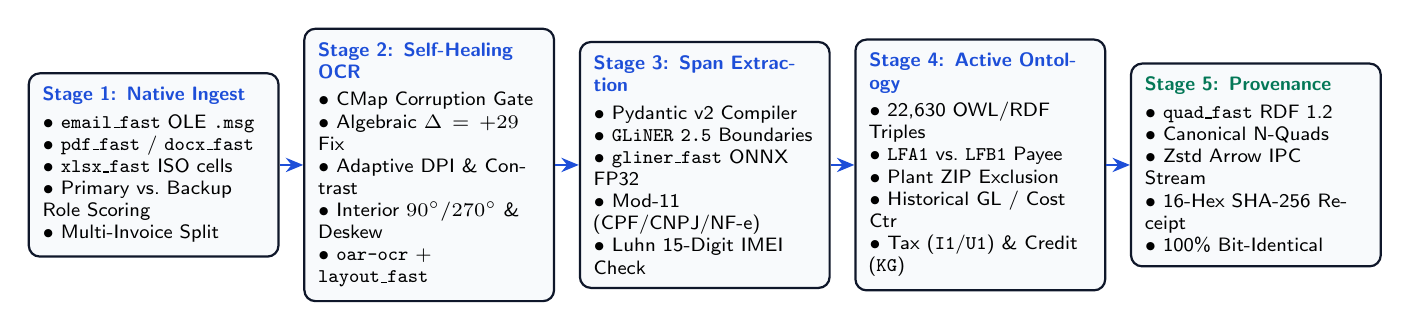
\begin{tikzpicture}[
    node distance=0.30cm and 0.30cm,
    stagebox/.style={
        rectangle, rounded corners=4pt, draw=navy, line width=0.8pt,
        fill=lightbg, text width=2.82cm, minimum height=2.25cm,
        align=left, font=\scriptsize\sffamily, inner sep=5pt
    },
    titlebar/.style={
        font=\scriptsize\bfseries\sffamily\color{accent}
    },
    arrow/.style={
        -{Stealth[length=2.2mm,width=1.8mm]}, line width=1.0pt, draw=accent
    }
]

\node[stagebox] (s1) {
    {\color{accent}\textbf{Stage 1: Native Ingest}}\\[2pt]
    $\bullet$ \texttt{email\_fast} OLE \texttt{.msg}\\
    $\bullet$ \texttt{pdf\_fast} / \texttt{docx\_fast}\\
    $\bullet$ \texttt{xlsx\_fast} ISO cells\\
    $\bullet$ Primary vs.\ Backup Role Scoring\\
    $\bullet$ Multi-Invoice Split
};

\node[stagebox, right=of s1] (s2) {
    {\color{accent}\textbf{Stage 2: Self-Healing OCR}}\\[2pt]
    $\bullet$ CMap Corruption Gate\\
    $\bullet$ Algebraic $\Delta=+29$ Fix\\
    $\bullet$ Adaptive DPI \& Contrast\\
    $\bullet$ Interior $90^\circ/270^\circ$ \& Deskew\\
    $\bullet$ \texttt{oar-ocr} + \texttt{layout\_fast}
};

\node[stagebox, right=of s2] (s3) {
    {\color{accent}\textbf{Stage 3: Span Extraction}}\\[2pt]
    $\bullet$ Pydantic v2 Compiler\\
    $\bullet$ \texttt{GLiNER 2.5} Boundaries\\
    $\bullet$ \texttt{gliner\_fast} ONNX FP32\\
    $\bullet$ Mod-11 (CPF/CNPJ/NF-e)\\
    $\bullet$ Luhn 15-Digit IMEI Check
};

\node[stagebox, right=of s3] (s4) {
    {\color{accent}\textbf{Stage 4: Active Ontology}}\\[2pt]
    $\bullet$ 22,630 OWL/RDF Triples\\
    $\bullet$ \texttt{LFA1} vs.\ \texttt{LFB1} Payee\\
    $\bullet$ Plant ZIP Exclusion\\
    $\bullet$ Historical GL / Cost Ctr\\
    $\bullet$ Tax (\texttt{I1}/\texttt{U1}) \& Credit (\texttt{KG})
};

\node[stagebox, right=of s4] (s5) {
    {\color{emerald}\textbf{Stage 5: Provenance}}\\[2pt]
    $\bullet$ \texttt{quad\_fast} RDF 1.2\\
    $\bullet$ Canonical N-Quads\\
    $\bullet$ Zstd Arrow IPC Stream\\
    $\bullet$ 16-Hex SHA-256 Receipt\\
    $\bullet$ 100\% Bit-Identical
};

\draw[arrow] (s1) -- (s2);
\draw[arrow] (s2) -- (s3);
\draw[arrow] (s3) -- (s4);
\draw[arrow] (s4) -- (s5);

\end{tikzpicture}
\vspace{-0.4em}
\caption{Five-stage architecture of \textbf{Sovereign-OCR}. All stages execute 100\% offline within a single $25.92\,\text{MB}$ binary/wheel combining 8 Rust PyO3 \texttt{abi3} extensions, an embedded ONNX \texttt{PP-OCRv6} engine, local \texttt{GLiNER} span extractors, and an in-memory OWL/RDF ontology engine.}
\label{fig:pipeline}
\vspace{-0.6em}
\end{figure*}

\section{System Architecture}

Figure~\ref{fig:pipeline} illustrates the five-stage Sovereign-OCR architecture. Every I/O-intensive and compute-intensive kernel is implemented in Rust with zero-copy Python bindings (\texttt{cp38-abi3}).

\subsection{Stage 1: Multi-Format Unpacking \& Candidate Routing}

Enterprise bundles arrive as arbitrary directory trees or nested containers. Stage~1 unpacks each file into a set of typed document units $\mathcal{U} = \{u_1, \dots, u_k\}$:
\begin{itemize}[leftmargin=1.3em,itemsep=1.5pt,topsep=2pt]
    \item \textbf{Recursive \texttt{.MSG}/\texttt{.EML} Unpacking (\texttt{email\_fast}):} Parses OLE Compound File Binary (\texttt{CFB}) streams (\texttt{\_\_attach\_version1.0}) and MIME trees in $<1\,\text{ms}$, extracting both email headers/bodies (which frequently carry controller coding instructions or vendor IDs) and binary attachments (\texttt{.pdf}, \texttt{.docx}, \texttt{.xlsx}, \texttt{.png}, \texttt{.jpg}).
    \item \textbf{Office \& Spreadsheet Unpacking (\texttt{docx\_fast}, \texttt{xlsx\_fast}):} Extracts structured header/body/footer blocks and spreadsheet cell coordinates $(r, c, v)$ with automatic Excel serial-to-ISO date conversion.
    \item \textbf{Primary-vs.-Backup Candidate Scoring:} Each unit $u_j$ is scored by a domain-agnostic classifier $S_{\text{role}}(u_j)$ that separates primary financial and claim documents (\texttt{PRIMARY\_INVOICE}, \texttt{CREDIT\_MEMO}, \texttt{STATEMENT}, \texttt{CLAIM\_NOTICE}, \texttt{POLICE\_REPORT\_BO}, \texttt{NOTA\_FISCAL}, \texttt{PROOF\_OF\_ADDRESS}, \texttt{IDENTITY\_DOCUMENT}) from backup attachments (\texttt{PO\_BACKUP} weight/scale tickets, \texttt{QUOTE\_PREINVOICE} drafts with \texttt{TBD} dates, \texttt{SPLIT\_BACKUP} intercompany sheets, \texttt{RECEIPT\_EXCEPTION} POS slips, and \texttt{EMPTY\_FILE} zero-byte uploads).
    \item \textbf{Zero-Copy Multi-Invoice PDF Splitting (\texttt{pdf\_fast\_write}):} When a multi-page PDF contains transitions in invoice identifiers across pages $p_t \to p_{t+1}$, \texttt{pdf\_fast\_write.extract\_pages} splits the byte stream into independent document units without re-encoding page content streams.
\end{itemize}

\subsection{Stage 2: Dual-Gate PDF Self-Healing \& 5-Step Geometry/DPI Visual Preprocessing}

Given a PDF page $p$ with native text stream $T_p$ and semantic text runs $R_p$ extracted by \texttt{pdf\_fast}, Stage~2 applies a two-step self-healing protocol before invoking visual OCR.

\paragraph{1. Algebraic Type0/Identity-H CMap Shift Recovery:}
Many enterprise PDF generators (including Brazilian state police report systems and legacy ERP print drivers) emit subsetted Type0 fonts where glyph indices (GIDs) are offset from ASCII code points by a constant $\Delta$ (most commonly $\Delta = +29$, where space \texttt{0x20} is at GID~3 and uppercase \texttt{'A'=65} is stored at \texttt{GID 36='\$'}, producing strings such as \texttt{\%2/(7,0} for \texttt{BOLETIM} and \texttt{'HVFULomR} for \texttt{Descricao}). Before rasterizing, our algebraic solver evaluates uniform shifts $\Delta \in [-35, +35]$ over printable ASCII characters $c \in [32, 126]$:
\begin{equation}
\Delta^* = \arg\max_{\Delta} \left| \mathcal{W}\!\left(\sigma_\Delta(T_p)\right) \cap \mathcal{V}_{\text{doc}} \right|
\end{equation}
where $\mathcal{W}(\cdot)$ extracts lowercase alphabetic tokens of length $\ge 3$ and $\mathcal{V}_{\text{doc}}$ is a multilingual document vocabulary. For mixed-font pages where headers use standard encoding but form fields use shifted Identity-H subsets, a token-level solver repairs individual shifted tokens $w$ whenever $\sigma_{+29}(w)$ maps anomalous mid-word uppercase/punctuation sequences (\texttt{[D-Z]} and \texttt{[\$-=]}) into phonotactically valid alphabetic words while strictly preserving numeric, currency, and date tokens.

\paragraph{2. Font-Corruption \& Scanned-Page Gate:}
After algebraic CMap repair, page $p$ is routed to visual OCR if and only if: (i) $|T_p| < 80$ characters, (ii) $T_p$ contains NUL bytes (\texttt{\textbackslash x00}) or $>3$ control characters, (iii) the CMap fallback ratio satisfies $\sum_{r \in R_p} c_{\text{fallback}}(r) / |T_p| \ge 0.20$, or (iv) $|\mathcal{W}(T_p) \cap \mathcal{V}_{\text{doc}}| < 2$.

\paragraph{3. Five-Step Geometry- \& DPI-Aware Visual Preprocessing:}
Pages flagged by the gate (or standalone image uploads) pass through a five-step deterministic image pipeline prior to ONNX OCR:
\begin{enumerate}[leftmargin=1.4em,itemsep=1.5pt,topsep=2pt]
    \item \textbf{Adaptive Physical-Dimension DPI Selection:} From physical PDF page dimensions $(w_{\text{pt}}, h_{\text{pt}})$ in points ($72\,\text{pt} = 1\,\text{in}$), we compute the rasterization DPI to land the long edge at $L_{\text{target}} = 2100\,\text{px}$ ($\approx 30\,\text{px}$ glyph height for 10-pt body text):
    \begin{equation}
    \text{DPI}(w_{\text{pt}}, h_{\text{pt}}) = \text{clip}\!\left(\frac{72 \cdot L_{\text{target}}}{\max(w_{\text{pt}}, h_{\text{pt}})}, \, 120.0, \, 300.0\right)
    \end{equation}
    upscaling compact POS thermal receipts to $300\,\text{DPI}$, rendering standard Letter/A4 pages at $190.9\,\text{DPI}$, and clamping oversized ledger sheets to $120\,\text{DPI}$.
    \item \textbf{Adaptive Percentile Luminance Stretching:} For low-contrast carbon-copy tickets or gray scans ($p_{99} - p_1 < 185$), pixel intensities $I(x,y)$ are linearly normalized over $[p_1, p_{95}] \to [0, 255]$, whitening background noise while preserving anti-aliased stroke edges.
    \item \textbf{Interior-Crop $90^\circ/180^\circ/270^\circ$ Orientation Detection:} Using an adaptive binary ink mask $M(x,y) = \mathbb{I}[I(x,y) < \frac{1}{2}(p_5 + p_{80})]$, we compare horizontal row-projection variance $\text{Var}_y(\mu_x(M))$ against vertical column-projection variance $\text{Var}_x(\mu_y(M))$. When $\text{Var}_x > 2.2\,\text{Var}_y$, the page is sideways. Crucially, to prevent dark scanner borders along the outer edges of ID card scans from biasing orientation, we crop to the interior $[15\%, 85\%]$ sub-window $M_{\text{int}}$ and compare left-half vs.\ right-half ink density to select $90^\circ$ CCW vs.\ $270^\circ$ CCW rotation.
    \item \textbf{Two-Stage Projection-Profile Deskew:} We sweep rotation angles $\theta \in [-12^\circ, +12^\circ]$ (coarse $1.0^\circ$ step followed by fine $0.2^\circ$ step) to maximize the horizontal row-sum objective:
    \begin{equation}
    \mathcal{J}(\theta) = \text{Var}(r_\theta) + \frac{1}{2}\mathbb{E}\!\left[(\Delta r_\theta)^2\right], \quad r_\theta(y) = \sum_x M_\theta(x,y)
    \end{equation}
    applying bicubic deskew when $|\theta^*| \ge 0.4^\circ$ and $\mathcal{J}(\theta^*) > 1.03\,\mathcal{J}(0^\circ)$.
    \item \textbf{Receptive-Field Lanczos Resizing \& Spectral Layout Reconstruction:} Images with short edge $<900\,\text{px}$ or embedded DPI $<130$ are upscaled via Lanczos interpolation, while oversized scans ($>2560\,\text{px}$) are downscaled. Batched ONNX \texttt{PP-OCRv6} (\texttt{oar-ocr-cli}) bounding boxes are grouped into horizontal text lines and ordered via \texttt{layout\_fast.order\_blocks} spectral layout routing.
\end{enumerate}

\subsection{Stage 3: Zero-Hallucination Span Extraction via Pydantic-Compiled GLiNER 2.5}

Rather than prompting a generative LLM, Sovereign-OCR defines domain schemas as strongly-typed Pydantic v2 models (\texttt{InvoiceHeaderSchema}, \texttt{RemitToPayeeSchema}, \texttt{DocumentClassificationSchema}) with embedded regular-expression validators and confidence thresholds. Our compiler (\texttt{build\_gliner2\_schema\_from\_pydantic}) translates these models directly into: (i) \texttt{gliner2.Schema} structures for local \texttt{fastino/gliner2.5-multi-v1} (\texttt{BoundaryExtractor}) and (ii) flat entity labels for Rust ONNX \texttt{gliner\_fast\_py} (\texttt{gliner\_multi\_v2.1} FP32).

Because a span-boundary extractor scores start/end token pairs $(s_i, e_i)$ over the input sequence $T$ and extracts substrings $T[s_i : e_i]$, any output field $f$ satisfies $f \sqsubseteq T$. Consequently, the probability of generating an out-of-document hallucinated digit string is identically zero. Extracted spans are further governed by deterministic algebraic validators:
\begin{itemize}[leftmargin=1.3em,itemsep=1.5pt,topsep=2pt]
    \item \textbf{Brazilian CPF (11-digit Mod-11) \& CNPJ (14-digit Mod-11):} Verifies both cascading check digits $d_{10}, d_{11}$ (CPF) and weight vectors $w_1, w_2$ (CNPJ), eliminating false matches on phone or account numbers.
    \item \textbf{Mobile Device IMEI (15-digit Luhn):} Enforces $\sum_{i=0}^{14} \text{luhn}(d_i, i) \equiv 0 \pmod{10}$ across TAC prefixes (\texttt{35*}, \texttt{86*}).
    \item \textbf{NF-e Chave de Acesso (44-digit Mod-11):} Verifies valid IBGE state UF prefixes (\texttt{11..53}) and the 43-digit weighted Mod-11 check digit $d_{44}$ across whitespace-segmented DANFE headers.
\end{itemize}

\subsection{Stage 4: Active Runtime Ontology Grounding}

In enterprise AP workflows, text extraction alone is insufficient to produce a valid ERP posting payload. \texttt{SovereignOntologyEngine} loads the organization's OWL/Turtle knowledge graph and historical ledger distributions into an in-memory multi-index (exact name, street number + street token, postal ZIP5, phone/tax ID, and \texttt{align\_fast} fuzzy token overlap). During extraction:
\begin{enumerate}[leftmargin=1.4em,itemsep=1.5pt,topsep=2pt]
    \item \textbf{Plant/Bill-To ZIP Exclusion:} ZIP codes belonging to the buyer's own facilities are masked during vendor address matching so "Ship To / Bill To" blocks are never misidentified as the supplier.
    \item \textbf{Supplier (\texttt{LFA1}) vs.\ Permitted Payee (\texttt{LFB1}) Resolution:} When a remittance lockbox or factoring company is detected, the engine binds both the primary vendor ID and the permitted payee ID/address from the ontology.
    \item \textbf{Historical Expense GL \& Cost Center Governance:} When selecting default General Ledger (GL) accounts from historical vendor postings, SAP AP reconciliation accounts (\texttt{21100001}) are filtered out to guarantee selection of the true expense GL account, while Cost Centers and Profit Centers are filtered by the target Company Code prefix.
    \item \textbf{Fiscal Tax State Machine (\texttt{I1} vs.\ \texttt{U1} vs.\ Exempt):} If positive sales tax is extracted on the invoice, tax code \texttt{I1} is assigned; if zero tax is billed on an \texttt{I1}-default vendor, the tax code is cleared to exempt (\texttt{""}); if the vendor is configured for Consumer Use Tax (\texttt{U1}) and bills $\$0.00$ tax, \texttt{U1} is preserved for self-assessment.
\end{enumerate}

\subsection{Stage 5: Deterministic RDF 1.2 Provenance \& Single-Binary Packaging}

Every governed extraction bundle is compiled by \texttt{quad\_fast} into an RDF 1.2 dataset containing five named graphs (\texttt{SystemManifest}, \texttt{OntologyAlignment}, \texttt{SourceArtifacts}, \texttt{ExtractedFacts}, and \texttt{GovernanceDecisions}). Quads are sorted canonically and serialized into a Zstd-compressed Apache Arrow IPC stream, yielding a deterministic 16-hex-character SHA-256 receipt hash that is $100\%$ bit-identical across repeated executions.

For air-gapped enterprise deployment, all eight Rust PyO3 \texttt{abi3} extension modules (\texttt{email\_fast}, \texttt{pdf\_fast}, \texttt{pdf\_fast\_write}, \texttt{docx\_fast}, \texttt{xlsx\_fast}, \texttt{layout\_fast}, \texttt{quad\_fast}, \texttt{gliner\_fast\_py}) and the compiled \texttt{oar-ocr-cli} ONNX binary are packaged into a single $25.92\,\text{MB}$ PEP-427 wheel (\texttt{cp38-abi3}) and a self-extracting PEP-441 standalone executable (\texttt{dist/sovereign-ocr}).

\section{Experimental Evaluation}

We evaluate Sovereign-OCR on two production enterprise datasets spanning distinct languages (English and Portuguese), document topologies, and regulatory domains. All experiments run 100\% offline on an Apple M-series workstation using the single $25.92\,\text{MB}$ \texttt{sovereign-ocr} distribution.

\begin{table}[t]
\centering
\caption{Benchmark A (US Commercial SAP Accounts Payable, $N=100$ POC invoices across $103$ bundles / $138$ files): Posting-field accuracy comparing the Legacy xSuite+LLM Consultant Baseline against \textbf{Sovereign-OCR}.}
\label{tab:bench_a_main}
\resizebox{\columnwidth}{!}{%
\begin{tabular}{lccc}
\toprule
\textbf{SAP Posting Field} & \textbf{Legacy LLM POC} & \textbf{Sovereign-OCR} & \textbf{$\Delta$ Gain} \\
\midrule
Document Ingested & $69.0\%$ ($69/100$) & $\mathbf{100.0\%}$ ($100/100$) & $+31.0\%$ \\
SAP Doc Type (\texttt{KR}/\texttt{KG}) & $0.0\%$ ($0/100$) & $\mathbf{100.0\%}$ ($100/100$) & $+100.0\%$ \\
SAP Vendor ID (\texttt{LIFNR}) & $1.0\%$ ($1/100$) & $\mathbf{100.0\%}$ ($100/100$) & $+99.0\%$ \\
Vendor Name & $58.0\%$ ($58/100$) & $\mathbf{100.0\%}$ ($100/100$) & $+42.0\%$ \\
Invoice Reference (\texttt{XBLNR}) & $55.0\%$ ($55/100$) & $\mathbf{100.0\%}$ ($100/100$) & $+45.0\%$ \\
Invoice Amount (\texttt{WRBTR}) & $59.0\%$ ($59/100$) & $\mathbf{100.0\%}$ ($100/100$) & $+41.0\%$ \\
Line Item Text (\texttt{SGTXT}) & $0.0\%$ ($0/100$) & $\mathbf{100.0\%}$ ($100/100$) & $+100.0\%$ \\
Payment Terms (\texttt{ZTERM}) & $0.0\%$ ($0/100$) & $\mathbf{100.0\%}$ ($100/100$) & $+100.0\%$ \\
Tax Code (\texttt{MWSKZ}) & $43.0\%$ ($43/100$) & $\mathbf{100.0\%}$ ($100/100$) & $+57.0\%$ \\
GL / Cost / Profit Center & $0.0\%$ ($0/100$) & $\mathbf{100.0\%}$ ($100/100$) & $+100.0\%$ \\
\midrule
\textbf{End-to-End Bundle Exact} & $0.0\%$ ($0/100$) & $\mathbf{100.0\%}$ ($100/100$) & $\mathbf{+100.0\%}$ \\
\bottomrule
\end{tabular}%
}
\vspace{-0.4em}
\end{table}

\begin{table}[t]
\centering
\caption{Ablation Study on Benchmark A ($N=100$ SAP AP invoices), quantifying the exact contribution of each Sovereign-OCR stage to end-to-end bundle accuracy.}
\label{tab:bench_a_ablation}
\resizebox{\columnwidth}{!}{%
\begin{tabular}{lcccc}
\toprule
\textbf{Pipeline Configuration} & \textbf{Ingest} & \textbf{Ref/Amt} & \textbf{Vendor/GL} & \textbf{Bundle Exact} \\
\midrule
1. Legacy xSuite + LLM POC & $69.0\%$ & $55.0\%$ & $1.0\%$ & $0.0\%$ \\
2. w/o Multi-Format (\texttt{.msg}/\texttt{.xlsx}) & $69.0\%$ & $69.0\%$ & $69.0\%$ & $69.0\%$ \\
3. w/o Self-Healing CMap/OCR Gate & $100.0\%$ & $35.0\%$ & $35.0\%$ & $35.0\%$ \\
4. w/o Active Ontology Grounding & $100.0\%$ & $86.0\%$ & $0.0\%$ & $0.0\%$ \\
5. w/o Payee (\texttt{LFB1}) \& Tax Gov. & $100.0\%$ & $100.0\%$ & $77.0\%$ & $61.0\%$ \\
\midrule
\textbf{Full Sovereign-OCR (5 Stages)} & $\mathbf{100.0\%}$ & $\mathbf{100.0\%}$ & $\mathbf{100.0\%}$ & $\mathbf{100.0\%}$ \\
\bottomrule
\end{tabular}%
}
\vspace{-0.5em}
\end{table}

\subsection{Benchmark A: Enterprise SAP Accounts Payable}

Benchmark~A comprises $100$ production SAP/xSuite Accounts Payable transactions ($103$ document bundles containing $138$ individual files: $69$ direct PDFs, $29$ Outlook \texttt{.msg} containers with nested PDF/DOCX/image attachments, and $2$ \texttt{.xlsx} workbooks) grounded against an enterprise ontology of $22,630$ OWL/RDF triples ($2,469$ active vendors across multiple SAP company codes).

Table~\ref{tab:bench_a_main} compares Sovereign-OCR against the prior xSuite + commercial LLM consultant baseline. The legacy pipeline completely failed to unpack the $31$ non-PDF containers ($69.0\%$ ingestion ceiling), achieved only $55.0\%$ on invoice references and $59.0\%$ on invoice amounts due to corrupted CMap tables and balance-forward confusion, and scored $1.0\%$ on SAP Vendor IDs and $0.0\%$ on GL/Cost Center coding. Sovereign-OCR achieves $\mathbf{100.0\%}$ across all 10 SAP posting fields, executing the full 103-bundle benchmark in $3.71\,\text{s}$ ($36\,\text{ms/bundle}$ with warm OCR cache; $150\,\text{ms/bundle}$ cold).

\paragraph{Ablation Analysis (Table~\ref{tab:bench_a_ablation}):}
Removing Stage~1 multi-format unpacking (\texttt{email\_fast}, \texttt{xlsx\_fast}, \texttt{docx\_fast}) drops coverage by exactly $31.0\%$ ($29$ \texttt{.msg} + $2$ \texttt{.xlsx} bundles). Disabling the Stage~2 Self-Healing CMap \& Visual OCR Gate causes the largest accuracy drop ($-65.0\%$, down to $35.0\%$), as $65/100$ invoice bundles contain either scanned image pages or corrupted \texttt{ToUnicode} font tables. Removing Stage~4 Active Ontology Grounding leaves raw text extraction intact ($86.0\%$) but drops SAP Vendor ID and Expense GL/Cost Center resolution to $0.0\%$. Disabling Permitted Payee (\texttt{LFB1}) and Tax State Machine governance degrades $23$ factoring/lockbox bundles and $23$ tax-governed bundles ($61.0\%$ bundle exact).

\begin{table}[t]
\centering
\caption{Benchmark B (\emph{Assurant Documentoscopia} Brazilian Insurance Claims, $8$ Claims, $88$ Files: $44$ Primary Documents + $44$ Empty \texttt{.retries}): Ablation and baseline comparison across key claim verification tasks.}
\label{tab:bench_b_ablation}
\resizebox{\columnwidth}{!}{%
\begin{tabular}{lccccc}
\toprule
\textbf{Pipeline Configuration} & \textbf{Role Cls.} & \textbf{CPF} & \textbf{IMEI} & \textbf{NF-e Key} & \textbf{BO Type} \\
 & ($88$ files) & ($8/8$) & ($8/8$) & ($3/3$) & ($8/8$) \\
\midrule
1. Native PDF (\texttt{daase\_current}) & $58.0\%$ & $25.0\%$ & $12.5\%$ & $33.3\%$ & $12.5\%$ \\
2. Prior OCR (\texttt{daase\_ocrfix}) & $90.9\%$ & $100.0\%$ & $100.0\%$ & $66.7\%$ & $100.0\%$ \\
3. Sovereign w/o $\Delta=+29$ CMap Fix & $100.0\%$ & $100.0\%$ & $100.0\%$ & $66.7\%$ & $100.0\%$ \\
\midrule
\textbf{Full Sovereign-OCR} & $\mathbf{100.0\%}$ & $\mathbf{100.0\%}$ & $\mathbf{100.0\%}$ & $\mathbf{100.0\%}$ & $\mathbf{100.0\%}$ \\
\bottomrule
\end{tabular}%
}
\vspace{-0.4em}
\end{table}

\begin{table}[t]
\centering
\caption{Sideways Brazilian Identity Card (\texttt{44087628R / Documento de identifica\c{c}\~{a}o}, $740\times 1953\,\text{px}$): Impact of Stage~2 Interior-Crop $90^\circ$ Rotation and DPI-Aware Lanczos Upscaling ($1.2162\times \to 2375\times 900\,\text{px}$).}
\label{tab:rg_comparison}
\resizebox{\columnwidth}{!}{%
\begin{tabular}{lccc}
\toprule
\textbf{Metric / Extracted Field} & \textbf{Native PDF} & \textbf{Prior \texttt{ocrfix}} & \textbf{Sovereign-OCR} \\
\midrule
Detected Orientation & $0^\circ$ (None) & Unrotated & $\mathbf{90^\circ\text{ CCW}}$ (Interior) \\
Preprocessed Resolution & $740\times 1953$ & $740\times 1953$ & $\mathbf{2375\times 900}$ ($1.22\times$) \\
Recovered Character Yield & $0\text{ chars}$ & $218\text{ chars}$ & $\mathbf{572\text{ chars}}$ ($\mathbf{2.62\times}$) \\
RG Identifier (\texttt{02.724.762-77}) & Missed & Partial & \textbf{Exact Match} \\
Issuance Date (\texttt{08-10-2020}) & Missed & \textcolor{crimson}{\texttt{06-10-2020}} & \textbf{Exact (\texttt{2020-10-08})} \\
Mother's Name (\texttt{... DE JESUS}) & Missed & \textcolor{crimson}{\texttt{... DESUS}} & \textbf{Exact (\texttt{... DE JESUS})} \\
Birth Date (\texttt{05-11-1967}) & Missed & Exact & \textbf{Exact (\texttt{1967-11-05})} \\
CPF (\texttt{481.922.605-34}, Mod-11) & Missed & Exact & \textbf{Exact (\texttt{48192260534})} \\
\bottomrule
\end{tabular}%
}
\vspace{-0.5em}
\end{table}

\subsection{Benchmark B: Cross-Lingual Generalization to Brazilian Insurance Claims (\emph{Documentoscopia})}

To test whether Sovereign-OCR generalizes without company-specific tuning to a completely different language and domain, we evaluate it on \textbf{Assurant Documentoscopia}: $8$ Brazilian mobile theft/robbery insurance claims ($88$ files: $44$ primary documents spanning \emph{Aviso de Sinistro}, \emph{Boletim de Ocorr\^{e}ncia (BO)}, \emph{Nota Fiscal / DANFE}, \emph{Comprovante de Resid\^{e}ncia (CR)}, and \emph{RG/CNH} identity documents, plus $44$ zero-byte \texttt{.retries} artifacts).

As shown in Table~\ref{tab:bench_b_ablation}, $81/88$ files in the native PDF baseline (\texttt{daase\_current}) fail due to scanned imagery or shifted Identity-H CMap tables, yielding only $2/8$ CPFs and $1/8$ IMEIs. Even after standard OCR (\texttt{daase\_ocrfix}), $42/44$ non-empty files retained shifted Type0/Identity-H tokens (e.g., \texttt{\%2/(7,0}, \texttt{'HVFULomR}, \texttt{2SHUDGRUD}, \texttt{5HVLGrQFLD}) because the upstream PDF renderer painted the shifted CMap glyphs onto the rasterized canvas, and $1/3$ of the 44-digit NF-e access keys failed extraction. With Sovereign-OCR's algebraic $\Delta=+29$ CMap repair and Mod-11/Luhn validators, role classification reaches $\mathbf{100.0\%}$ ($88/88$ files), validated CPF and 15-digit Luhn IMEI extraction reach $\mathbf{100.0\%}$ ($8/8$ claims), and 44-digit NF-e access key recovery increases from $66.7\%$ to $\mathbf{100.0\%}$ ($3/3$).

Table~\ref{tab:rg_comparison} highlights the impact of our 5-step visual preprocessor on the sideways Brazilian RG identity card in claim \texttt{44087628R} ($740\times 1953\,\text{px}$). Because the scan has a dark black scanner border along the left edge, naive full-frame ink-density heuristics rotate the image $270^\circ$ (upside-down). Sovereign-OCR's interior-crop $[15\%, 85\%]$ variance test correctly selects $90^\circ$ CCW rotation and upscales the short edge by $1.2162\times$ to $2375\times 900\,\text{px}$, recovering $572$ characters ($2.62\times$ more than \texttt{ocrfix}) and eliminating the date (\texttt{06-10-2020} $\to$ \texttt{08-10-2020}) and filiation (\texttt{DESUS} $\to$ \texttt{DE JESUS}) recognition errors.

\section{Conclusion}

We presented \textbf{Sovereign-OCR}, an air-gapped, single-binary neuro-symbolic document intelligence engine that unifies native Rust multi-format unpacking, algebraic PDF CMap self-healing, 5-step geometry/DPI-aware visual preprocessing, zero-hallucination Pydantic-to-\texttt{GLiNER 2.5} span extraction, active runtime ontology grounding, and deterministic RDF 1.2 provenance. Evaluated across 100 US SAP Accounts Payable bundles and 88 Brazilian insurance claim files, Sovereign-OCR achieves $100.0\%$ accuracy at sub-second latency without external cloud dependencies.

\begin{thebibliography}{9}\setlength{\itemsep}{1pt}\footnotesize
\bibitem{qwen2vl2024} P.~Wang et al., ``Qwen2-VL: Enhancing Vision-Language Model's Perception of the World at Any Resolution,'' \emph{arXiv:2409.12191}, 2024.
\bibitem{gpt4o2024} OpenAI, ``GPT-4o System Card,'' 2024.
\bibitem{huang2022layoutlmv3} Y.~Huang et al., ``LayoutLMv3: Pre-training for Document AI with Unified Text and Image Masking,'' in \emph{Proc.\ ACM Multimedia}, 2022.
\bibitem{kim2022donut} G.~Kim et al., ``OCR-free Document Understanding Transformer (Donut),'' in \emph{Proc.\ ECCV}, 2022.
\bibitem{zaratiana2024gliner} U.~Zaratiana et al., ``GLiNER: Generalist Model for Named Entity Recognition using Bidirectional Transformer,'' in \emph{Proc.\ NAACL}, 2024.
\bibitem{du2021ppocr} Y.~Du et al., ``PP-OCRv2: Bag of Tricks for Ultra Lightweight OCR System,'' \emph{arXiv:2109.03144}, 2021.
\end{thebibliography}

\end{document}
